%
% $RCSfile: paper.tex,v $
%
% Copyright (c) 2001-2004. Christian Heller. All rights reserved.
%
% No copying, altering, distribution or any other actions concerning this
% document, except after explicit permission by the author!
% At some later point in time, this document is planned to be put under
% the GNU FDL license. For now, _everything_ is _restricted_ by the author.
%
% http://www.cybop.net
% - Cybernetics Oriented Programming -
%
% http://www.resmedicinae.org
% - Information in Medicine -
%
% @author Christian Heller <christian.heller@tuxtax.de>
%

%
% The document class specifying the type of document.
%
\documentclass[a4paper,10pt]{llncs}

%
% The usepackages for document class.
%

% Paper format and font.
\usepackage{a4,times,helvet}

% Graphics.
\usepackage{graphicx}

%
% The space settings for edges (left, top, right, bottom).
%
\setlength{\hoffset}{-3,9cm}
\setlength{\voffset}{-3,6cm}
\setlength{\oddsidemargin}{4cm}
\setlength{\evensidemargin}{3cm}
\setlength{\topmargin}{1,5cm}
\setlength{\textwidth}{17cm}
\setlength{\textheight}{25cm}

%
% The hyphenation list.
%
%
% $RCSfile: hyphenation.tex,v $
%
% Copyright (c) 2002-2007. Christian Heller. All rights reserved.
%
% Permission is granted to copy, distribute and/or modify this document
% under the terms of the GNU Free Documentation License, Version 1.1 or
% any later version published by the Free Software Foundation; with no
% Invariant Sections, with no Front-Cover Texts and with no Back-Cover
% Texts. A copy of the license is included in the section entitled
% "GNU Free Documentation License".
%
% http://www.cybop.net
% - Cybernetics Oriented Programming -
%
% Version: $Revision: 1.2 $ $Date: 2007-08-01 13:59:00 $ $Author: christian $
% Authors: Christian Heller <christian.heller@tuxtax.de>
%

\hyphenation{abs-trac-tion}
\hyphenation{ac-tu-ally}
\hyphenation{ana-lyst}
\hyphenation{ana-ly-sis}
\hyphenation{an-cient}
\hyphenation{ap-pli-ca-tion}
\hyphenation{aris-to-tle}
\hyphenation{at-tri-bute}
\hyphenation{be-ing}
\hyphenation{ca-te-go-ri-za-tion}
\hyphenation{client}
\hyphenation{com-po-nen-ti-za-tion}
\hyphenation{com-pu-ter}
\hyphenation{con-fi-gure}
\hyphenation{con-nec-ted}
\hyphenation{cy-ber-ne-tics}
\hyphenation{cyboi}
\hyphenation{cybol}
\hyphenation{cybop}
\hyphenation{des-cribed}
\hyphenation{de-sign}
\hyphenation{de-ve-lop-ment}
\hyphenation{dis-crete}
\hyphenation{di-vide}
\hyphenation{do-main}
\hyphenation{dy-na-mic}
\hyphenation{eli-mi-nate}
\hyphenation{eli-mi-nates}
\hyphenation{eli-mi-na-tion}
\hyphenation{en-gi-nee-ring}
\hyphenation{en-vi-ron-ment}
\hyphenation{ex-pert}
\hyphenation{fi-gure}
\hyphenation{fle-xi-bi-li-sie-rung}
\hyphenation{fun-da-men-tal}
\hyphenation{hard-ware}
\hyphenation{hu-man}
\hyphenation{im-ple-men-ta-tion}
\hyphenation{in-he-rit}
\hyphenation{in-he-ri-tance}
\hyphenation{in-ter-pre-ter}
\hyphenation{java}
\hyphenation{know-ledge}
\hyphenation{lan-guage}
\hyphenation{li-ving}
\hyphenation{lo-gi-cal}
\hyphenation{ma-na-ge-ment}
\hyphenation{mea-ning-ful}
\hyphenation{me-cha-nism}
\hyphenation{me-mo-ry}
\hyphenation{me-thod}
\hyphenation{me-thods}
\hyphenation{mo-del-ling}
\hyphenation{na-ture}
\hyphenation{net-work}
\hyphenation{neu-ral}
\hyphenation{neu-ron}
\hyphenation{ne-ver-en-ding-ly}
\hyphenation{open}
\hyphenation{operating}
\hyphenation{ori-en-ted}
\hyphenation{over-come}
\hyphenation{par-ti-cu-lar}
\hyphenation{prin-ci-ple}
\hyphenation{pro-ba-bi-lis-tic}
\hyphenation{pro-ble-ma-tic}
\hyphenation{pro-gram-ming}
\hyphenation{res-pon-sible}
\hyphenation{re-u-sa-bi-li-ty}
\hyphenation{sci-ence}
\hyphenation{server}
\hyphenation{si-mi-lar}
\hyphenation{soft-ware}
\hyphenation{source}
\hyphenation{spe-cia-li-za-tion}
\hyphenation{spe-ci-fied}
\hyphenation{sta-tic}
\hyphenation{sta-ti-cally}
\hyphenation{sto-chas-tic}
\hyphenation{stone-on-stone}
\hyphenation{struc-ture}
\hyphenation{strug-gling}
\hyphenation{subs-ti-tu-ting}
\hyphenation{su-per-flu-ous}
\hyphenation{sup-ply-ing}
\hyphenation{sys-tem}
\hyphenation{taeu-schungs-ver-such}
\hyphenation{temp-lates}
\hyphenation{tes-ting}
\hyphenation{thin-king}
\hyphenation{un-en-li-vened}
\hyphenation{un-sa-tis-fy-ing}
\hyphenation{va-ry-ing}
\hyphenation{weigh-ted}
\hyphenation{zu-kunfts-si-che-re}


%
% This document is a scientific paper to be handed in for a conference.
%
% @version $Revision: 1.1 $ $Date: 2004-04-27 10:43:02 $ $Author: christian $
% @author Christian Heller <christian.heller@tuxtax.de>
% @author Christian Heller <christian.heller@tu-ilmenau.de>
%
\begin{document}
    \twocolumn
    \title{Flexible Software Architectures for Presentation Layers demonstrated on Medical Documentation with Episodes and Inclusion of Topological Report}
\author{Jens Bohl \(<\)info@jens-bohl.de\(>\)\\
Torsten Kunze \(<\)zone3@gmx.de\(>\)\\
Christian Heller \(<\)christian.heller@tu-ilmenau.de\(>\)\\
Ilka Philippow \(<\)ilka.philippow@tu-ilmenau.de\(>\)}
\institute{
Technical University of Ilmenau\\
Faculty for Computer Science and Automation\\
Institute for Theoretical and Technical Informatics\\
PF 100565, Max-Planck-Ring 14, 98693 Ilmenau, Germany\\
http://www.tu-ilmenau.de, fon: +49-(0)3677-69-1230, fax: +49-(0)3677-69-1220}
\maketitle

    \maketitle
    %
% $RCSfile: abstract.tex,v $
%
% Copyright (c) 2001-2004. Christian Heller. All rights reserved.
%
% No copying, altering, distribution or any other actions concerning this
% document, except after explicit permission by the author!
% At some later point in time, this document is planned to be put under
% the GNU FDL license. For now, _everything_ is _restricted_ by the author.
%
% http://www.cybop.net
% - Cybernetics Oriented Programming -
%
% http://www.resmedicinae.org
% - Information in Medicine -
%
% @author Christian Heller <christian.heller@tuxtax.de>
%

\begin{abstract}
This article reports about an ongoing research investigating the possibilities
for applying inter-disciplinary concepts to software system design. The new
resulting programming philosophy is based on firstly, a distinction of statics
and dynamics, secondly a knowledge schema structuring models and their meta
information hierarchically, and thirdly the separation of state- and logic
knowledge. It solves many of the problems existing in classical programming
paradigms and languages and may have the potential to replace these in the long
run.\\
\textbf{Keywords:} Knowledge Abstraction, Cybernetics Oriented Programming,
CYBOP, Software Design
\end{abstract}

    %
% $RCSfile: introduction.tex,v $
%
% Copyright (c) 2002-2007. Christian Heller. All rights reserved.
%
% Permission is granted to copy, distribute and/or modify this document
% under the terms of the GNU Free Documentation License, Version 1.1 or
% any later version published by the Free Software Foundation; with no
% Invariant Sections, with no Front-Cover Texts and with no Back-Cover
% Texts. A copy of the license is included in the section entitled
% "GNU Free Documentation License".
%
% http://www.cybop.net
% - Cybernetics Oriented Programming -
%
% Version: $Revision: 1.1 $ $Date: 2007-07-17 20:02:36 $ $Author: christian $
% Authors: Christian Heller <christian.heller@tuxtax.de>
%

\chapter{Introduction}
\label{introduction_heading}
\index{Introduction}

This is just a test \cite{zimmermann} citation.

%
% $RCSfile: terminology.tex,v $
%
% Copyright (C) 2002-2008. Christian Heller.
%
% Permission is granted to copy, distribute and/or modify this document
% under the terms of the GNU Free Documentation License, Version 1.1 or
% any later version published by the Free Software Foundation; with no
% Invariant Sections, with no Front-Cover Texts and with no Back-Cover
% Texts. A copy of the license is included in the section entitled
% "GNU Free Documentation License".
%
% http://www.cybop.net
% - Cybernetics Oriented Programming -
%
% http://www.resmedicinae.org
% - Information in Medicine -
%
% Version: $Revision: 1.1 $ $Date: 2008-08-19 20:41:09 $ $Author: christian $
% Authors: Christian Heller <christian.heller@tuxtax.de>
%

\subsection{Terminology}
\label{terminology_heading}
\index{Terminology}
\index{Lexicon}
\index{Vocabulary}
\index{Nomenclature}
\index{Hierarchy}
\index{Semantic Link}
\index{Directed Acyclic Graph}
\index{DAG}

While a \emph{Lexicon} is a list of pure words, a \emph{Terminology} (sometimes
called \emph{Vocabulary}) can also contain phrases. Because it is a fixed list
of lots of terms, a terminology should exclude any link to a separate list of
concepts. When a terminology contains additional instructions describing how to
interpret each term, or dictating when to choose one over another
(prioritisation), it may be called a \emph{Nomenclature}. The knowledge schema
proposed in this work (chapter \ref{knowledge_schema_heading}) shall be capable
of storing codes of various terminology systems.

Lexicon and terminology stand for a \emph{Set} of words or terms, respectively.
To bring some structure into such a set, terms or concepts need to be ordered,
that is organised through a system of links, into a \emph{Hierarchy}, which
Rogers \cite{rogers} defines as a:

\begin{quote}
    \ldots\ tree-like structure, where things at the top of the tree are in some
    way more general or abstract than the things lower down. The nature of each
    link between each level in the tree may be explicit or only implied, and
    more than one flavour of semantic link can be used to build the tree (in
    which case it may be called a \emph{Mixed Hierarchy}).
\end{quote}

Kinds of hierarchies, as means of organisation, are:

\begin{itemize}
    \item[-] \emph{Subsumption Hierarchy} (Classification, Taxonomy): only
        \emph{is-a} relationships exist between parent-child pairs in the tree
    \item[-] \emph{Uniaxial Hierarchy:} each concept only ever has one parent,
        though it can have more than one child
    \item[-] \emph{Multiaxial Hierachy:} each concept can have more than one
        parent as well as more than one child
    \item[-] \emph{Exhaustive Multiaxial Hierarchy:} all concepts have all the
        parents as well as all the children they should have
\end{itemize}

As organisation \emph{Rules} count:

\begin{itemize}
    \item[-] \emph{Formalism}: an explicitly expressed set of rules, like the
        specification for how to tell what should (not) be a parent of a concept
    \item[-] \emph{Concept System} (Model): a system of \emph{Symbols} that
        stand in for concepts and/ or the links between them, and which may or
        may not be intended to be processed with reference to some formalism
    \item[-] \emph{Partonomy} (Mereology): a system of concepts and links
        intended to represent whole-part relationships specifically
\end{itemize}

On a yet higher abstract level, a \emph{Data Structure} may hold organisations
of concepts. Various types of data structures are:

\begin{itemize}
    \item[-] \emph{Network}: a mesh-like structure that connects terms or concepts
        using links; a hierarchy can be thought of as simple case of a network
    \item[-] \emph{Graph}: a network
    \item[-] \emph{Directed Graph}: a network in which each link has a \emph{Direction}
    \item[-] \emph{Directed Acyclic Graph} (DAG): a directed graph free of loops
\end{itemize}

A knowledge template expressed in the language that will be defined in chapter
\ref{cybernetics_oriented_language_heading} describes an uniaxial hierarchy,
that is its sub concepts have just one parent node. Its structure follows the
partonomy (mereology) organisation rules and represents a DAG.

%
% $RCSfile: cybernetics_oriented_programming.tex,v $
%
% Copyright (c) 2002-2007. Christian Heller. All rights reserved.
%
% Permission is granted to copy, distribute and/or modify this document
% under the terms of the GNU Free Documentation License, Version 1.1 or
% any later version published by the Free Software Foundation; with no
% Invariant Sections, with no Front-Cover Texts and with no Back-Cover
% Texts. A copy of the license is included in the section entitled
% "GNU Free Documentation License".
%
% http://www.cybop.net
% - Cybernetics Oriented Programming -
%
% Version: $Revision: 1.1 $ $Date: 2007-07-17 20:02:36 $ $Author: christian $
% Authors: Christian Heller <christian.heller@tuxtax.de>
%

\section{Cybernetics Oriented Programming}
\label{cybernetics_oriented_programming_heading}
\index{Cybernetics Oriented Programming}

The \emph{Cybernetics Oriented Programming} (CYBOP) software development theory
suggests to ...

%
% $RCSfile: software_engineering_process.tex,v $
%
% Copyright (c) 2002-2007. Christian Heller. All rights reserved.
%
% Permission is granted to copy, distribute and/or modify this document
% under the terms of the GNU Free Documentation License, Version 1.1 or
% any later version published by the Free Software Foundation; with no
% Invariant Sections, with no Front-Cover Texts and with no Back-Cover
% Texts. A copy of the license is included in the section entitled
% "GNU Free Documentation License".
%
% http://www.cybop.net
% - Cybernetics Oriented Programming -
%
% Version: $Revision: 1.1 $ $Date: 2007-07-17 20:02:36 $ $Author: christian $
% Authors: Christian Heller <christian.heller@tuxtax.de>
%

\subsection{Software Engineering Process}
\label{software_engineering_process_heading}
\index{Software Engineering Process}

Although hundreds of variations, with or without iterations, exist, a standard
\emph{Software Engineering Process} (SEP) consists of the phases: \emph{Analysis},
\emph{Design} and \emph{Implementation}, as illustrated in figure
\ref{software_engineering_process_figure}.

\begin{figure}[ht]
    \begin{center}
        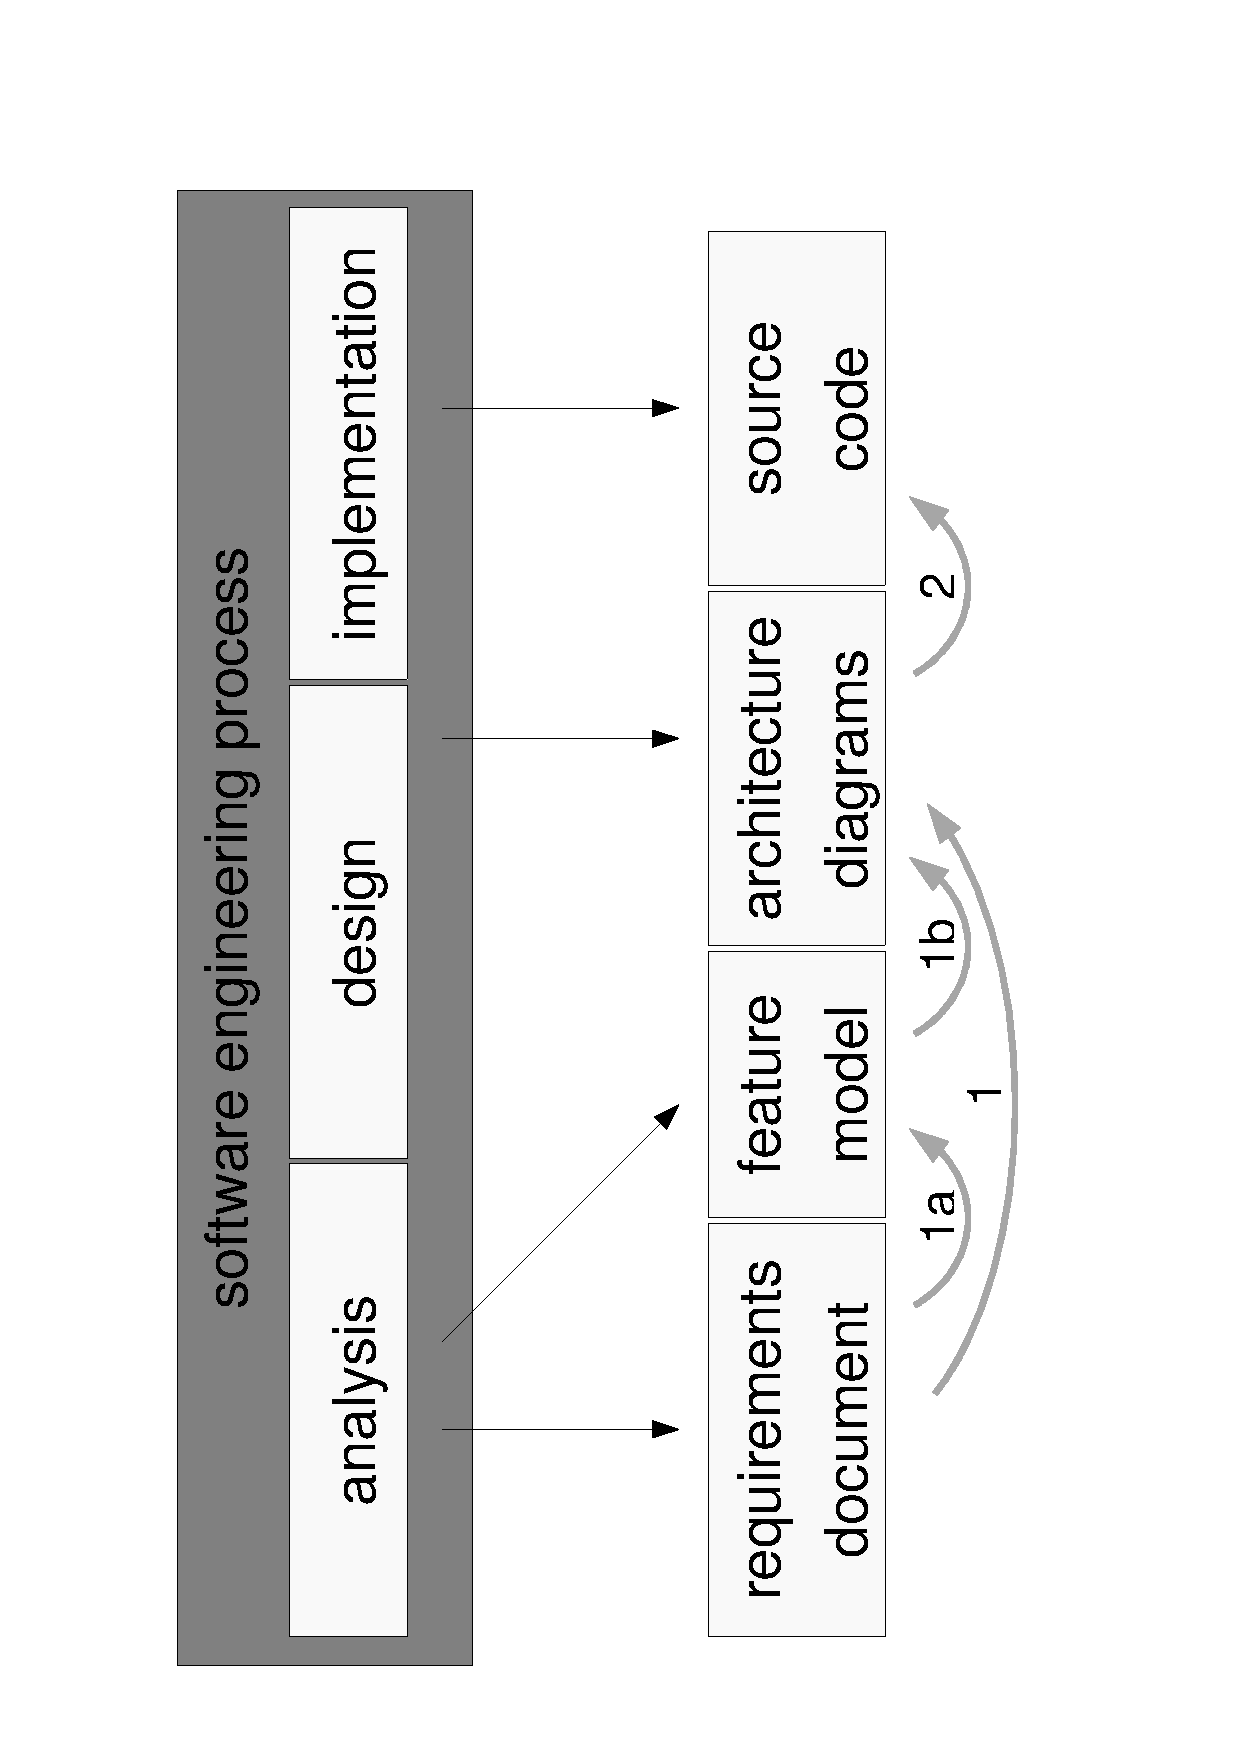
\includegraphics[scale=0.3,angle=-90]{graphics/gaps.pdf}
        \caption{Standard Software Engineering Process}
        \label{software_engineering_process_figure}
    \end{center}
\end{figure}

%
% $RCSfile: interpretation.tex,v $
%
% Copyright (c) 2002-2007. Christian Heller. All rights reserved.
%
% Permission is granted to copy, distribute and/or modify this document
% under the terms of the GNU Free Documentation License, Version 1.1 or
% any later version published by the Free Software Foundation; with no
% Invariant Sections, with no Front-Cover Texts and with no Back-Cover
% Texts. A copy of the license is included in the section entitled
% "GNU Free Documentation License".
%
% http://www.cybop.net
% - Cybernetics Oriented Programming -
%
% Version: $Revision: 1.1 $ $Date: 2007-07-17 20:02:36 $ $Author: christian $
% Authors: Christian Heller <christian.heller@tuxtax.de>
%

\subsection{Interpretation}
\label{inerpretation_heading}
\index{Interpretation}

CYBOP
CYBOL
CYBOI

\begin{figure}[ht]
    \begin{center}
        \includegraphics[scale=0.3,angle=-90]{graphics/connection.pdf}
        \caption{CYBOL Interpretation}
        \label{cybol_interpretation_figure}
    \end{center}
\end{figure}


%
% $RCSfile: extensible_markup_language.tex,v $
%
% Copyright (c) 2002-2007. Christian Heller. All rights reserved.
%
% Permission is granted to copy, distribute and/or modify this document
% under the terms of the GNU Free Documentation License, Version 1.1 or
% any later version published by the Free Software Foundation; with no
% Invariant Sections, with no Front-Cover Texts and with no Back-Cover
% Texts. A copy of the license is included in the section entitled
% "GNU Free Documentation License".
%
% http://www.cybop.net
% - Cybernetics Oriented Programming -
%
% Version: $Revision: 1.1 $ $Date: 2007-07-17 20:02:36 $ $Author: christian $
% Authors: Christian Heller <christian.heller@tuxtax.de>
%

\section{Extensible Markup Language}
\label{extensible_markup_language_heading}
\index{Extensible Markup Language}

The \emph{Extensible Markup Language} (XML) is ...


    %
% $RCSfile: software_engineering_process.tex,v $
%
% Copyright (c) 2002-2007. Christian Heller. All rights reserved.
%
% Permission is granted to copy, distribute and/or modify this document
% under the terms of the GNU Free Documentation License, Version 1.1 or
% any later version published by the Free Software Foundation; with no
% Invariant Sections, with no Front-Cover Texts and with no Back-Cover
% Texts. A copy of the license is included in the section entitled
% "GNU Free Documentation License".
%
% http://www.cybop.net
% - Cybernetics Oriented Programming -
%
% Version: $Revision: 1.1 $ $Date: 2007-07-17 20:02:36 $ $Author: christian $
% Authors: Christian Heller <christian.heller@tuxtax.de>
%

\subsection{Software Engineering Process}
\label{software_engineering_process_heading}
\index{Software Engineering Process}

Although hundreds of variations, with or without iterations, exist, a standard
\emph{Software Engineering Process} (SEP) consists of the phases: \emph{Analysis},
\emph{Design} and \emph{Implementation}, as illustrated in figure
\ref{software_engineering_process_figure}.

\begin{figure}[ht]
    \begin{center}
        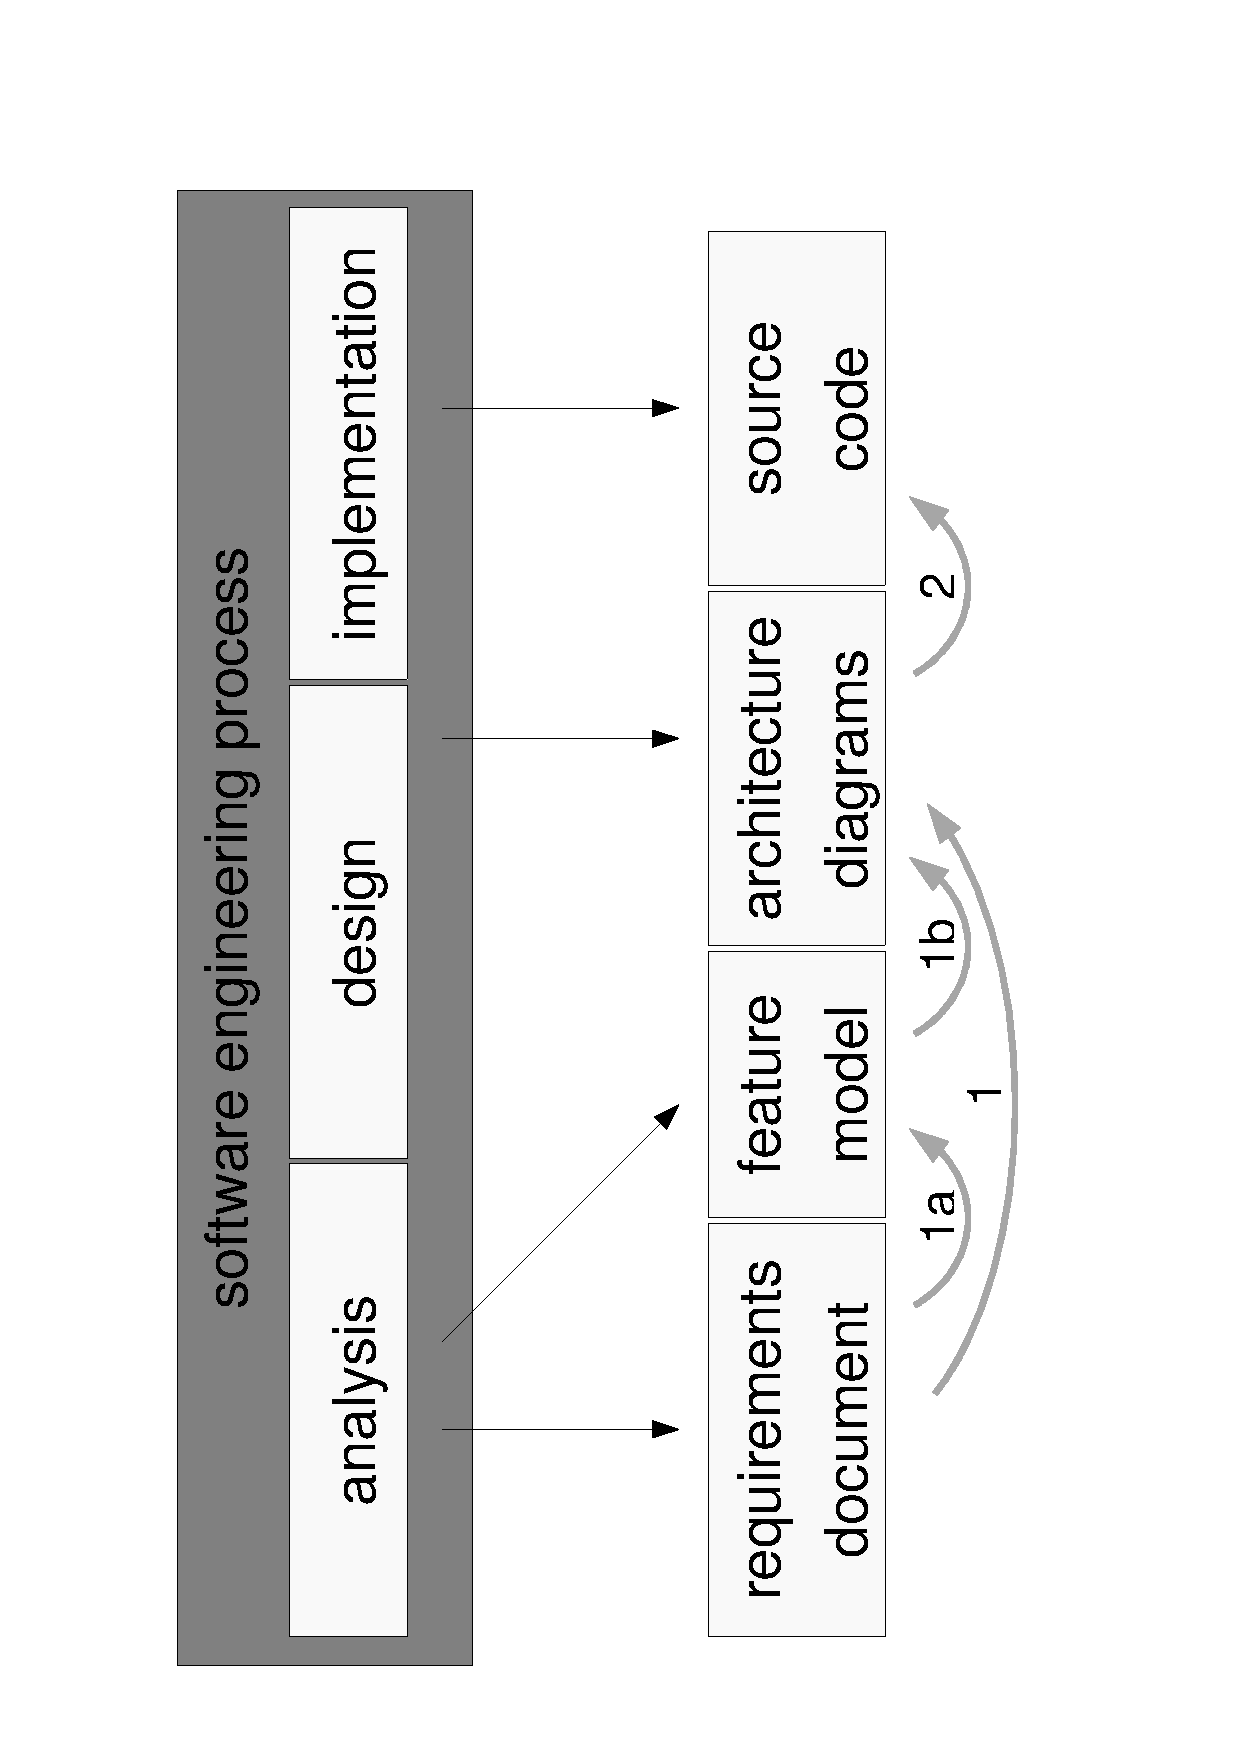
\includegraphics[scale=0.3,angle=-90]{graphics/gaps.pdf}
        \caption{Standard Software Engineering Process}
        \label{software_engineering_process_figure}
    \end{center}
\end{figure}

    %
% $RCSfile: traditional_programming.tex,v $
%
% Copyright (c) 2001-2004. Christian Heller. All rights reserved.
%
% No copying, altering, distribution or any other actions concerning this
% document, except after explicit permission by the author!
% At some later point in time, this document is planned to be put under
% the GNU FDL license. For now, _everything_ is _restricted_ by the author.
%
% http://www.cybop.net
% - Cybernetics Oriented Programming -
%
% http://www.resmedicinae.org
% - Information in Medicine -
%
% @author Christian Heller <christian.heller@tuxtax.de>
%

\section{Traditional Programming}
\label{traditional_programming_heading}

Section \ref{software_engineering_process_heading} pointed out a problem that all
current software engineering processes are struggling with: \emph{Abstraction Gaps}.
To find out about possible reasons, traditional and current programming concepts
need to be inspected closer.

%
% $RCSfile: property_bundling.tex,v $
%
% Copyright (c) 2001-2004. Christian Heller. All rights reserved.
%
% No copying, altering, distribution or any other actions concerning this
% document, except after explicit permission by the author!
% At some later point in time, this document is planned to be put under
% the GNU FDL license. For now, _everything_ is _restricted_ by the author.
%
% http://www.cybop.net
% - Cybernetics Oriented Programming -
%
% http://www.resmedicinae.org
% - Information in Medicine -
%
% @author Christian Heller <christian.heller@tuxtax.de>
%

\subsection{Property Bundling}
\label{property_bundling_heading}

Software consists of data which can be processed by a computer. This is possible
because \emph{qualitative} data are transformed into \emph{quantitative} data and,
finally, to \emph{Zero} and \emph{One}. \emph{Mathematics} delivers the \emph{Logic}
(\emph{Operations}) after which \emph{States} (\emph{Operands}) can be mapped,
to deliver the expected results.

When combining a number of operations in a certain order, an \emph{Algorithm} is
retrieved. The operands it works with are stored in \emph{Variables}. As can be
seen, there is always \emph{static} and \emph{dynamic} structures involved, the
static holding the states and the dynamic holding the rules for mapping between
states.

\emph{Structured}/ \emph{Procedural Programming} languages were the first to
explicitly provide the means to model static \emph{Structures} as well as dynamic
\emph{Procedures} (or \emph{Functions}, respectively). Both can be cascaded in
\emph{Hierarchies} and even use \emph{Recursion} for that.

Yet other synonyms for static and dynamic structures that were introduced by the
nowadays more popular \emph{Object Oriented Programming} (OOP) are \emph{Attribute}
and \emph{Method}. Both can be properties of an \emph{Object} which is the runtime
instance of a \emph{Class} which in turn represents the data \emph{Type}. A class
can \emph{inherit} properties from a \emph{super} class. This \emph{Inheritance}
was a truely new and innovative concept brought in by OOP. The \emph{Bundling} of
static and dynamic properties (attributes and methods), on the other hand, causes
more system interdependencies and complications than were predictable. It is a big
disadvantage that affects all modern object-oriented systems.

Certainly, the bundling stems from best intentions to receive cleaner code by
keeping not only attributes but also methods in a common module, such avoiding
\emph{wild} and \emph{global} procedures. But now, modules not only had to refer
to other modules for accessing their data; the same was needed for accessing methods.
With OOP, the number of cross-relations between modules and system interdependencies
in general nearly always rise dramatically. In reality, static and dynamic
properties are two \emph{different} things that have to be kept in different
places! Both can have a similar, hierarchical structure but each is a concept on
its own.

\emph{Interface} inheritance is used to implement \emph{Concerns} in a system.
\emph{Aspect Oriented Programming} (AOP) calls its concerns \emph{Aspects} and
uses special language means to implement them. With standard class constellations,
\emph{Design Patterns} provide clear solutions describing how best to combine
(associate/ inherit) classes. As subsumption of many design patterns, a
\emph{Framework} aims to provide basic functionality for the applications to be
embedded into it. All these efforts are based upon OOP. The main idea behind them
is to prevent code duplication and to minimize the interdependencies between
parts of a system. But what if OOP is one reason for just those interdependencies?

Big systems with a multitude of associations and dependencies often lead to a
loss in overview which results in so called \emph{Spaghetti Code}.
\emph{Component Oriented Programming} (COP) tries to solve this by encapsulating
code in smaller \emph{Components} which shall make it easier to keep overview.
People started to dream about a simple combination of such components and called
it the \emph{LEGO Metapher} (with relation to the building blocks for children).
But software models are not simple building blocks that could be built
\emph{Stone-on-Stone}! They are concepts as known from \emph{Human Thinking}.

The components described to here are \emph{passive} because they need a system
to call them. More recent studies are about \emph{active} components, sometimes
called \emph{Agents}. These are self-acting processes that solve special tasks.
The concepts behind are called \emph{Agent Oriented Programming}.

Passive components and all of the programming concepts described before them
belong to the \emph{Logical Architecture} of a system. The term
\emph{Physical Architecture} is used when it comes to active components, agents,
processes or systems in general.

%
% $RCSfile: information_mix.tex,v $
%
% Copyright (c) 2001-2004. Christian Heller. All rights reserved.
%
% No copying, altering, distribution or any other actions concerning this
% document, except after explicit permission by the author!
% At some later point in time, this document is planned to be put under
% the GNU FDL license. For now, _everything_ is _restricted_ by the author.
%
% http://www.cybop.net
% - Cybernetics Oriented Programming -
%
% http://www.resmedicinae.org
% - Information in Medicine -
%
% @author Christian Heller <christian.heller@tuxtax.de>
%

\subsection{Information Mix}
\label{information_mix_heading}

Of course, the bundling of static and dynamic properties as used in OOP is not
the only factor causing interdependencies. Otherwise, traditional procedural
programming languages had already delivered ideal systems. But this is not the
case. Something else must be missing. The major problem of today's software is
its \emph{Mix} of two very different kinds of information: \emph{System Control}
and \emph{Application Knowledge}.

A standard computer architecture consists of a \emph{Memory} (which stores data),
a \emph{Processor} (that applies operations on the data), \emph{Input/Output Devices}
(to correspond with the environment) and a \emph{Bus System} (that connects the
before-mentioned parts). All these devices need to be controlled in some way.
Variable values (instances) need to be written to and read from the memory;
operations which the processor offers need to be called; input and output values
need to be exchanged through the corresponding input/output devices.

Most of this is done by an \emph{Operating System} (OS) and its hardware drivers.
However, programming languages allow their users to access hardware, too. Software
programmers can send processor instructions, they can allocate (instantiate)
memory etc. It is these possibilities which lead to memory leaks and further
software problems. If the operating system, for example, concentrated all memory
allocation in one place, forgotten instances would belong to the past.

The remaining code represents the actual \emph{Application}. It contains the
\emph{Domain Knowledge}, the \emph{Concepts}, the \emph{Configuration} information.
These models of real world phenomenons have nothing to do with hardware control
and need to be treated differently.


    %
% $RCSfile: human_thinking.tex,v $
%
% Copyright (c) 2004. Christian Heller. All rights reserved.
%
% No copying, altering, distribution or any other actions concerning this
% document, except after explicit permission by the author!
% At some later point in time, this document is planned to be put under
% the GNU FDL license. For now, _everything_ is _restricted_ by the author.
%
% http://www.cybop.net
% - Cybernetics Oriented Programming -
%
% http://www.resmedicinae.org
% - Information in Medicine -
%
% @author Christian Heller <christian.heller@tuxtax.de>
%

\subsection{Human Thinking}
\label{human_thinking_heading}

The new classification is based on the idea of categorizing software patterns
after the principles of \emph{Human Thinking}, that is concepts of the logical
\emph{Mind}, as opposed to \emph{Artificial Neural Networks} (ANN) that want to
imitate the functioning of the physical \emph{Brain}.

The corresponding concepts were first introduced in \cite{heller2004}. After an
investigation of the fundamentals of human thinking, that is how human beings
understand their surrounding real world by abstracting it in \emph{Models}, that
paper concludes that there were three basic activities of abstraction:

\begin{enumerate}
    \item Discrimination
    \item Categorization
    \item Composition
\end{enumerate}

By discriminating their environment, humans are able to share it into discrete
\emph{Items}. Items with similar properties can be classified into a common super
\emph{Category}. Any abstract model of the universe is just an illusion, being
made up of yet smaller models, and nobody knows where this hierarchy really stops,
towards microcosm as well as towards macrocosm. Therefore, the third and last
kind of abstraction, namely composition, lets humans perceive the items in their
environment as \emph{Compound} of smaller items.

\begin{figure}[ht]
    \begin{center}
        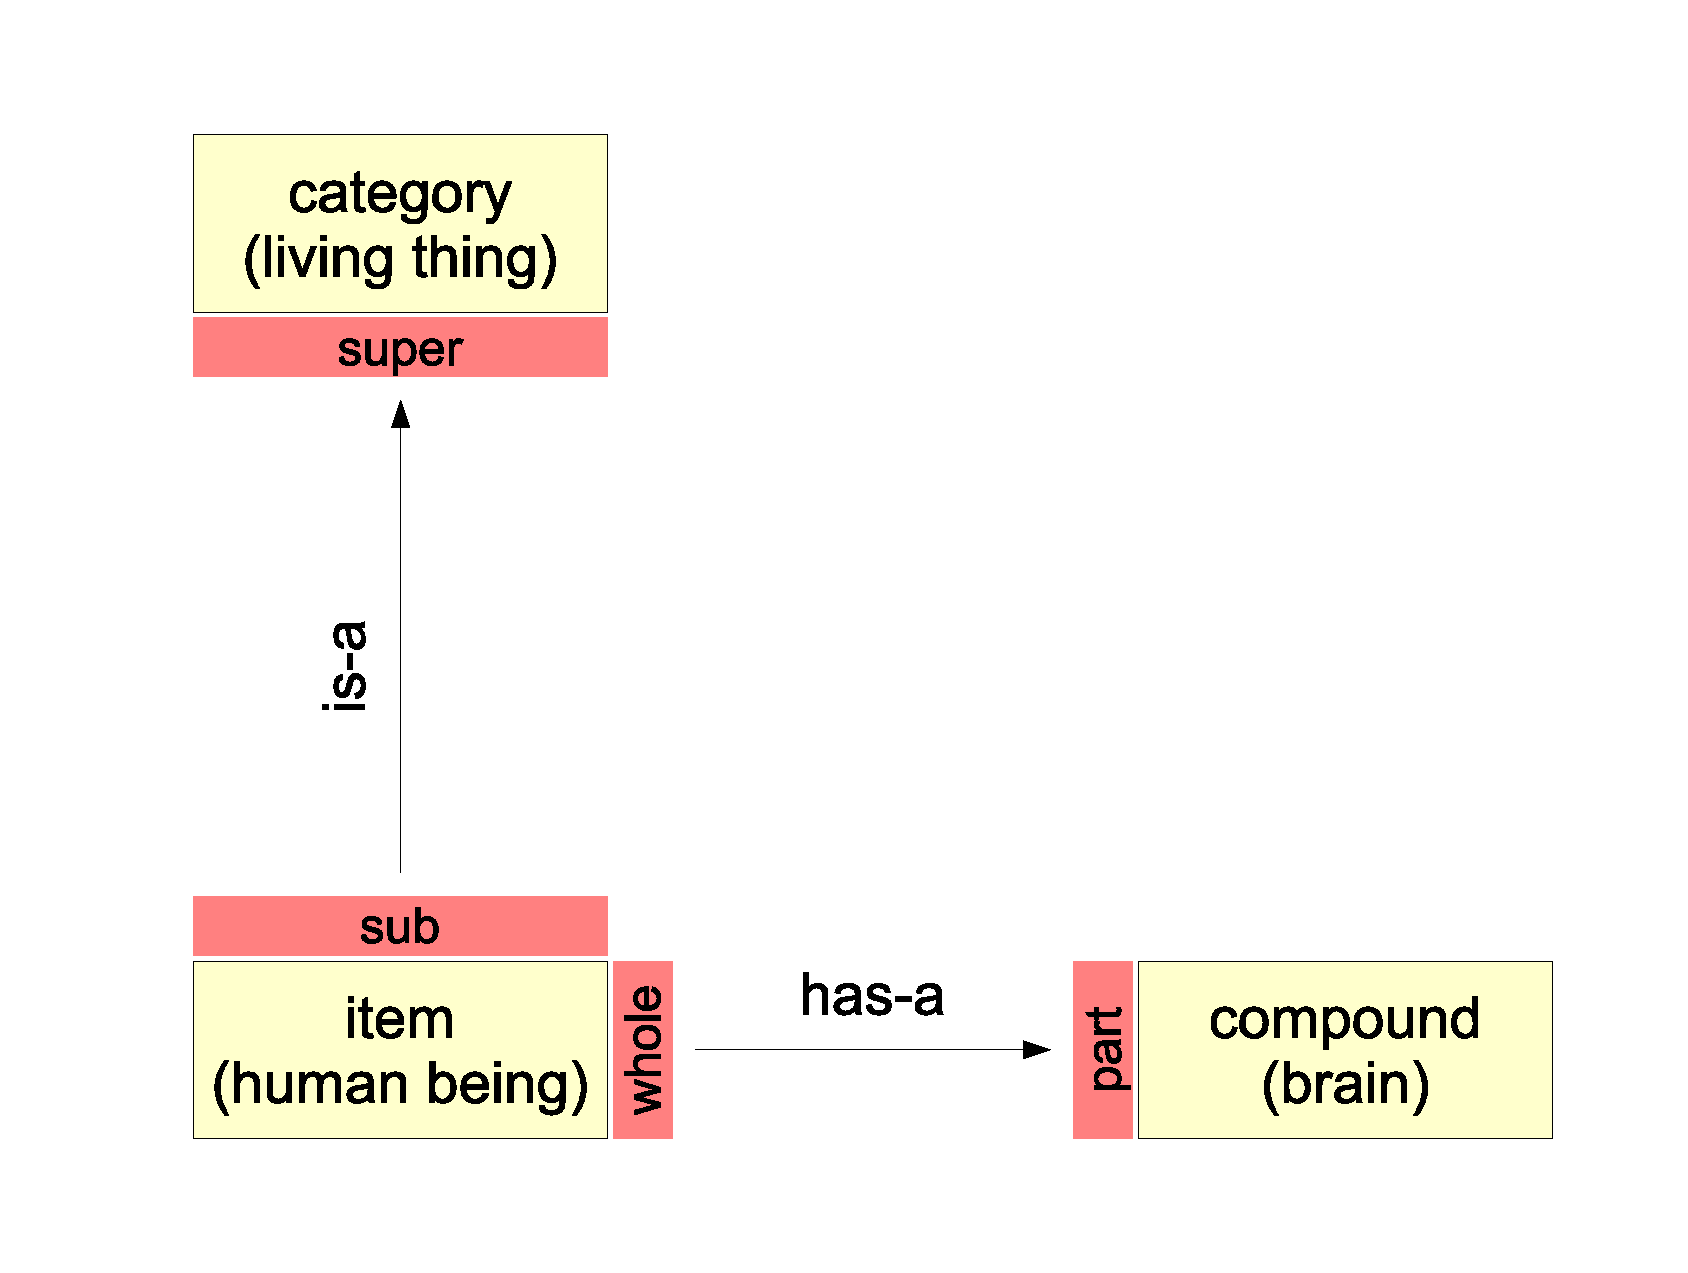
\includegraphics[scale=0.3]{vector/abstraction.eps}
        \caption{Abstractions of Human Thinking \cite{heller2004}}
        \label{abstraction_figure}
    \end{center}
\end{figure}

The latter two activities of abstraction -- categorization and composition --
are based on special \emph{Associations} (figure \ref{abstraction_figure}),
between a \emph{Super-} and a \emph{Sub} model and between a \emph{Whole-} and
a \emph{Part} model, respectively.

    %
% $RCSfile: cybernetics_oriented_language.tex,v $
%
% Copyright (c) 2001-2004. Christian Heller. All rights reserved.
%
% No copying, altering, distribution or any other actions concerning this
% document, except after explicit permission by the author!
% At some later point in time, this document is planned to be put under
% the GNU FDL license. For now, _everything_ is _restricted_ by the author.
%
% http://www.cybop.net
% - Cybernetics Oriented Programming -
%
% http://www.resmedicinae.org
% - Information in Medicine -
%
% @author Christian Heller <christian.heller@tuxtax.de>
%

\section{Cybernetics Oriented Language}
\label{cybernetics_oriented_language_heading}

The introduced \emph{Cybernetics Oriented Language} (CYBOL) is based on the
principles of \emph{Human Thinking} as described in section \ref{human_thinking_heading}.
These principles and further concepts behind are summarized by the name
\emph{Cybernetics Oriented Programming} (CYBOP) (figure \ref{cybop_figure}).
They form the semantics of CYBOL. Its syntax is determined by the \emph{Extensible
Markup Language} (XML) standard and accordingly easy. It is rich enough to express
models based upon the three kinds of abstraction: \emph{Discrimination},
\emph{Categorization} and \emph{Composition} as well as meta information of a
\emph{Whole} about its \emph{Parts}.

\begin{figure}[ht]
    \begin{center}
        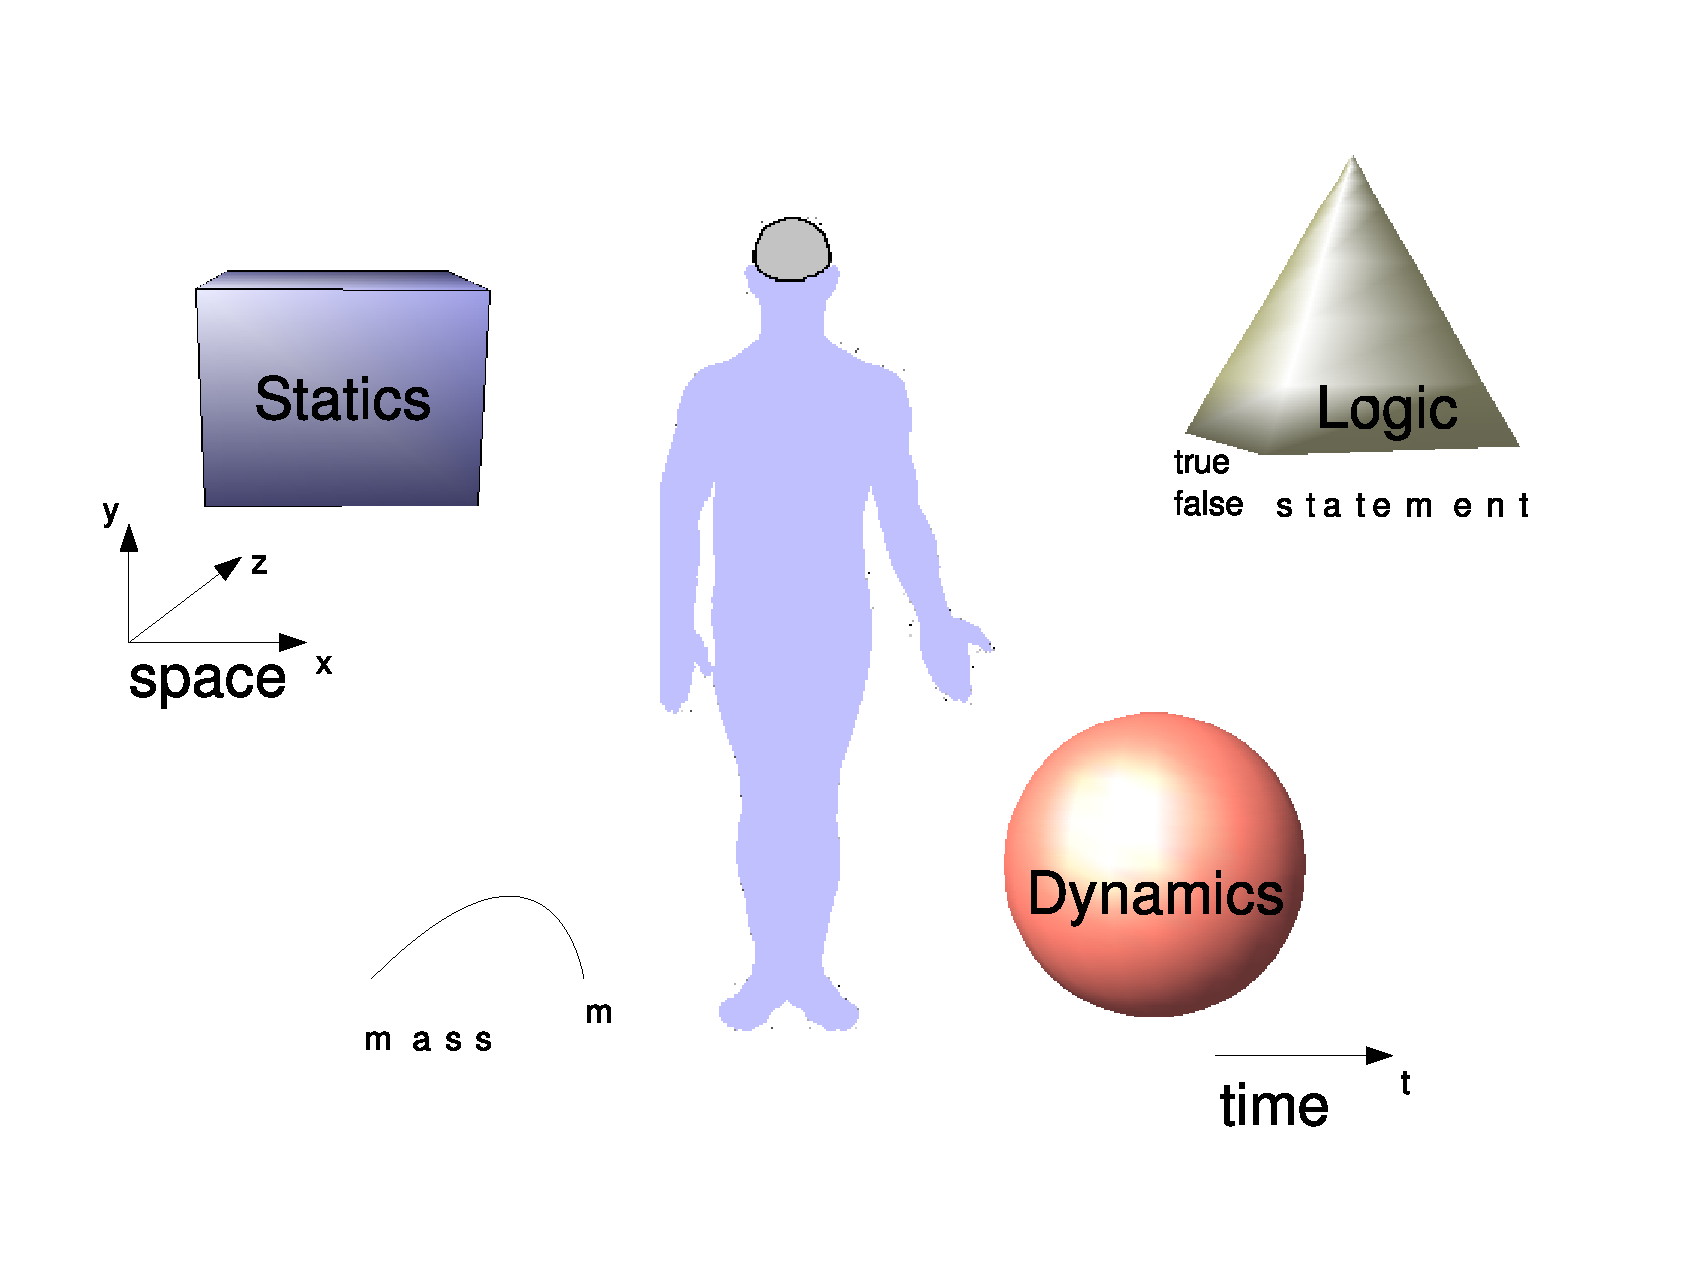
\includegraphics[scale=0.3]{vector/cybop.eps}
        \caption{CYBOP}
        \label{cybop_figure}
    \end{center}
\end{figure}

%
% $RCSfile: syntax.tex,v $
%
% Copyright (C) 2002-2008. Christian Heller.
%
% Permission is granted to copy, distribute and/or modify this document
% under the terms of the GNU Free Documentation License, Version 1.1 or
% any later version published by the Free Software Foundation; with no
% Invariant Sections, with no Front-Cover Texts and with no Back-Cover
% Texts. A copy of the license is included in the section entitled
% "GNU Free Documentation License".
%
% http://www.cybop.net
% - Cybernetics Oriented Programming -
%
% http://www.resmedicinae.org
% - Information in Medicine -
%
% Version: $Revision: 1.1 $ $Date: 2008-08-19 20:41:09 $ $Author: christian $
% Authors: Christian Heller <christian.heller@tuxtax.de>
%

\subsection{Syntax}
\label{syntax_heading}
\index{CYBOL Syntax}
\index{Syntax of a Language}
\index{Grammar of a Language}
\index{Extensible Markup Language}
\index{XML}
\index{XML Tag}
\index{XML Attribute}
\index{Discrimination}
\index{Composition}

Every language has a special \emph{Syntax}, that is a \emph{Grammar} with rules
for combining terms and symbols \cite{foldoc}. CYBOL could define its own
syntax or use an already existing one, of another language. Because of its
popularity, clear text representation, flexibility, extensibility and ease of
use, \emph{XML} was chosen to deliver the syntax for CYBOL.

To mention just two of the syntactical elements of XML, \emph{Tag} and
\emph{Attribute} are considered shortly here. Tags are special, arbitrary
keywords that have to be defined by the system working with an XML document.
Attributes keep additional information about the contents enclosed by two tags.
Two examples:

\begin{scriptsize}
    \begin{verbatim}
    <tag attribute="value">
        contents
    </tag>
    \end{verbatim}
\end{scriptsize}

\begin{scriptsize}
    \begin{verbatim}
    <tag attribute1="value" attribute2="contents"/>
    \end{verbatim}
\end{scriptsize}

An XML document carries a name and can such represent a \emph{Discrete Item},
as suggested by the principles of human thinking (section
\ref{human_thinking_heading}). Being a \emph{Compound}, it consists of parts --
and, it can link to other documents treated as its parts. That way, a whole
hierarchy can be formed. Tag attributes can keep additional information about
the linked parts. Most importantly, XML documents have a hierarchical structure
based on tags, which may be used to store meta information about a part.

Considering these properties of XML, it seems predestinated for formally
representing abstract models using the CYBOP concepts. CYBOL, finally, is XML
\emph{plus} a defined set of tags, attributes and values, used to structure and
link documents meaningfully.

%
% $RCSfile: vocabulary.tex,v $
%
% Copyright (C) 2002-2008. Christian Heller.
%
% Permission is granted to copy, distribute and/or modify this document
% under the terms of the GNU Free Documentation License, Version 1.1 or
% any later version published by the Free Software Foundation; with no
% Invariant Sections, with no Front-Cover Texts and with no Back-Cover
% Texts. A copy of the license is included in the section entitled
% "GNU Free Documentation License".
%
% http://www.cybop.net
% - Cybernetics Oriented Programming -
%
% http://www.resmedicinae.org
% - Information in Medicine -
%
% Version: $Revision: 1.1 $ $Date: 2008-08-19 20:41:09 $ $Author: christian $
% Authors: Christian Heller <christian.heller@tuxtax.de>
%

\subsection{Vocabulary}
\label{vocabulary_heading}
\index{CYBOL Vocabulary}
\index{Terms of a Language}
\index{Symbols of a Language}
\index{Syntax of a Language}
\index{Document Type Definition}
\index{DTD}
\index{XML Schema Definition}
\index{XSD}
\index{Extended Backus Naur Form}
\index{EBNF}

The \emph{Vocabulary} is what fills a language with life. It delivers the
\emph{Terms} and \emph{Symbols} that are combined after the rules of a syntax.

XML allows to define and exchange the whole vocabulary of a language. It offers
two ways in which a list of legal elements can be defined: The traditional
\emph{Document Type Definition} (DTD) and the more modern
\emph{XML Schema Definition} (XSD). Besides the vocabulary, DTD and XSD define
the structure of an XML document and allow to typify, constrain and validate
items. In addition to DTD and XSD, the \emph{Extended Backus Naur Form} (EBNF)
of CYBOL is given following.

The language definitions were not added as appendix to this work, because
firstly, they are not too long and secondly, an understanding of the CYBOL
elements is necessary to be able to grasp the constructs and examples given in
later sections.

%
% $RCSfile: document_type_definition.tex,v $
%
% Copyright (c) 2002-2007. Christian Heller. All rights reserved.
%
% Permission is granted to copy, distribute and/or modify this document
% under the terms of the GNU Free Documentation License, Version 1.1 or
% any later version published by the Free Software Foundation; with no
% Invariant Sections, with no Front-Cover Texts and with no Back-Cover
% Texts. A copy of the license is included in the section entitled
% "GNU Free Documentation License".
%
% http://www.cybop.net
% - Cybernetics Oriented Programming -
%
% Version: $Revision: 1.2 $ $Date: 2007-08-01 13:59:00 $ $Author: christian $
% Authors: Christian Heller <christian.heller@tuxtax.de>
%

\subsection{Document Type Definition}
\label{document_type_definition_heading}
\index{Document Type Definition}
\index{DTD}
\index{Extensible Markup Language}
\index{XML}
\index{Markup Tag}
\index{model Tag}
\index{part Tag}
\index{property Tag}
\index{constraint Tag}
\index{name Attribute}
\index{channel Attribute}
\index{abstraction Attribute}
\index{model Attribute}

A DTD represents the type definition of an XML document. It consists of a set
of \emph{Markup Tags} and their \emph{Interpretation} \cite{foldoc}. DTDs can
be declared inline, within a document, or as an external reference
\cite{w3schools}. Figure \ref{dtd_figure} shows the DTD of the CYBOL language.

\begin{figure}[ht]
    \bigskip
    \begin{scriptsize}
        \begin{verbatim}
<!ELEMENT model (part*)>
<!ELEMENT part (property*)>
<!ELEMENT property (constraint*)>
<!ELEMENT constraint EMPTY>

<!ATTLIST part
    name CDATA #REQUIRED
    channel CDATA #REQUIRED
    abstraction CDATA #REQUIRED
    model CDATA #REQUIRED>
<!ATTLIST property
    name CDATA #REQUIRED
    channel CDATA #REQUIRED
    abstraction CDATA #REQUIRED
    model CDATA #REQUIRED>
<!ATTLIST constraint
    name CDATA #REQUIRED
    channel CDATA #REQUIRED
    abstraction CDATA #REQUIRED
    model CDATA #REQUIRED>
        \end{verbatim}
    \end{scriptsize}
    \caption{Recommended CYBOL DTD}
    \label{dtd_figure}
\end{figure}

Following the pure hierarchical structure of CYBOL, it would actually suffice
to use a DTD as simple as the one shown in figure \ref{simpledtd_figure}. Since
the three elements \emph{part}, \emph{property} and \emph{constraint} (compare
figure \ref{dtd_figure}) have the same list of required attributes, they could
be summarised under the name \emph{part}, for example. Because the structure of
a CYBOL model is non-ambiguous, the meaning of its elements can be guessed from
their position within the model.

\begin{figure}[ht]
    \bigskip
    \begin{scriptsize}
        \begin{verbatim}
<!ELEMENT part (part*)>

<!ATTLIST part
    name CDATA #REQUIRED
    channel CDATA #REQUIRED
    abstraction CDATA #REQUIRED
    model CDATA #REQUIRED>
        \end{verbatim}
    \end{scriptsize}
    \caption{Simplified CYBOL DTD}
    \label{simpledtd_figure}
\end{figure}

\clearpage

For the purpose of expressing knowledge in accordance with the schema suggested
by CYBOP \cite{cybop}, a CYBOL knowledge template (file) does not need to have
a root element. The file name clearly identifies it. For reasons of XML
conformity, however, an extra root element called \emph{model} was defined
(figure \ref{dtd_figure}). And for reasons of better readability and
programmability, the three kinds of embedded elements were given distinct names.

\clearpage
%
% $RCSfile: xml_schema_definition.tex,v $
%
% Copyright (c) 2002-2007. Christian Heller. All rights reserved.
%
% Permission is granted to copy, distribute and/or modify this document
% under the terms of the GNU Free Documentation License, Version 1.1 or
% any later version published by the Free Software Foundation; with no
% Invariant Sections, with no Front-Cover Texts and with no Back-Cover
% Texts. A copy of the license is included in the section entitled
% "GNU Free Documentation License".
%
% http://www.cybop.net
% - Cybernetics Oriented Programming -
%
% Version: $Revision: 1.1 $ $Date: 2007-07-17 20:02:36 $ $Author: christian $
% Authors: Christian Heller <christian.heller@tuxtax.de>
%

\section{XML Schema Definition}
\label{xml_schema_definition_heading}
\index{XML Schema Definition}
\index{XSD}
\index{CYBOL XSD}
\index{XML Schema}
\index{Extensible Markup Language}
\index{XML}

\emph{XML Schema} is an XML-based alternative to DTD \cite{w3schools}, and XSD
is its definition language. There is a lot of discussion going on about the
sense or \emph{Myth} of XML Schema \cite{browne}, that this document will not
take part in. Figure \ref{xsd_figure} shows the XSD of the CYBOL language.

\begin{figure}[ht]
    \bigskip
    \bigskip
    \begin{scriptsize}
        \begin{verbatim}
<?xml version="1.0"?>
<xs:schema xmlns:xs='http://www.w3.org/2001/XMLSchema' targetNamespace='http://www.cybop.net'
    xmlns='http://www.cybop.net' elementFormDefault='qualified'>
    <xs:element name='part'>
        <xs:complexType>
            <xs:sequence>
                <xs:element ref='part' minOccurs='0' maxOccurs='unbounded'/>
            </xs:sequence>
            <xs:attribute name='name' type='xs:string' use='required'/>
            <xs:attribute name='channel' type='xs:string' use='required'/>
            <xs:attribute name='abstraction' type='xs:string' use='required'/>
            <xs:attribute name='model' type='xs:string' use='required'/>
        </xs:complexType>
    </xs:element>
</xs:schema>
        \end{verbatim}
    \end{scriptsize}
    \caption{Simplified CYBOL XSD}
    \label{simplexsd_figure}
\end{figure}

\begin{figure}[ht]
    \bigskip
    \bigskip
    \begin{scriptsize}
        \begin{verbatim}
<?xml version="1.0"?>
<xs:schema xmlns:xs='http://www.w3.org/2001/XMLSchema' targetNamespace='http://www.cybop.net'
    xmlns='http://www.cybop.net' elementFormDefault='qualified'>
    <xs:element name='model'>
        <xs:complexType>
            <xs:sequence>
                <xs:element ref='part' minOccurs='0' maxOccurs='unbounded'/>
            </xs:sequence>
        </xs:complexType>
    </xs:element>
    <xs:element name='part'>
        <xs:complexType>
            <xs:sequence>
                <xs:element ref='property' minOccurs='0' maxOccurs='unbounded'/>
            </xs:sequence>
            <xs:attribute name='name' type='xs:string' use='required'/>
            <xs:attribute name='channel' type='xs:string' use='required'/>
            <xs:attribute name='abstraction' type='xs:string' use='required'/>
            <xs:attribute name='model' type='xs:string' use='required'/>
        </xs:complexType>
    </xs:element>
    <xs:element name='property'>
        <xs:complexType>
            <xs:sequence>
                <xs:element ref='constraint' minOccurs='0' maxOccurs='unbounded'/>
            </xs:sequence>
            <xs:attribute name='name' type='xs:string' use='required'/>
            <xs:attribute name='channel' type='xs:string' use='required'/>
            <xs:attribute name='abstraction' type='xs:string' use='required'/>
            <xs:attribute name='model' type='xs:string' use='required'/>
        </xs:complexType>
    </xs:element>
    <xs:element name='constraint'>
        <xs:complexType>
            <xs:attribute name='name' type='xs:string' use='required'/>
            <xs:attribute name='channel' type='xs:string' use='required'/>
            <xs:attribute name='abstraction' type='xs:string' use='required'/>
            <xs:attribute name='model' type='xs:string' use='required'/>
        </xs:complexType>
    </xs:element>
</xs:schema>
        \end{verbatim}
    \end{scriptsize}
    \caption{Recommended CYBOL XSD}
    \label{xsd_figure}
\end{figure}

Again, a simplified version of that XSD could be created (figure
\ref{simplexsd_figure}). But for reasons explained before, the recommended XSD
is the one shown in figure \ref{xsd_figure}.

%
% $RCSfile: extended_backus_naur_form.tex,v $
%
% Copyright (C) 2002-2008. Christian Heller.
%
% Permission is granted to copy, distribute and/or modify this document
% under the terms of the GNU Free Documentation License, Version 1.1 or
% any later version published by the Free Software Foundation; with no
% Invariant Sections, with no Front-Cover Texts and with no Back-Cover
% Texts. A copy of the license is included in the section entitled
% "GNU Free Documentation License".
%
% http://www.cybop.net
% - Cybernetics Oriented Programming -
%
% http://www.resmedicinae.org
% - Information in Medicine -
%
% Version: $Revision: 1.1 $ $Date: 2008-08-19 20:41:06 $ $Author: christian $
% Authors: Christian Heller <christian.heller@tuxtax.de>
%

\subsubsection{Extended Backus Naur Form}
\label{extended_backus_naur_form_heading}
\index{Extended Backus Naur Form}
\index{EBNF}
\index{Backus Naur Form}
\index{BNF}
\index{CYBOL EBNF}

The EBNF adds regular expression syntax to the \emph{Backus Naur Form} (BNF)
notatation \cite{naur}, in order to allow very compact specifications
\cite{kuhn}. Figure \ref{ebnf_figure} shows the EBNF of the CYBOL language.

\begin{figure}[ht]
    \bigskip
    \bigskip
    \begin{scriptsize}
        \begin{verbatim}
CYBOL       = '<model>'
                    {part}
                '</model>';

part        = '<part ' attributes '\>' |
                '<part ' attributes '>'
                    {property}
                '</part>';

property    = '<property ' attributes '\>' |
                '<property ' attributes '>'
                    {constraint}
                '</property>';

constraint  = '<constraint ' attributes '\>';

attributes  = name_attribute channel_attribute abstraction_attribute model_attribute

name_attribute          = 'name="' name '"';
channel_attribute       = 'channel="' channel '"';
abstraction_attribute   = 'abstraction="' abstraction '"';
model_attribute         = 'model="' model '"';

name        = description_sign;
channel     = description_sign;
abstraction = description_sign;
model       = value_sign;

description_sign    = { ( letter | number ) };
value_sign          = { ( letter | number | other_sign ) };

letter          = small_letter | big_letter;
small_letter    = 'a' | 'b' | 'c' | 'd' | 'e' | 'f' | 'g' |
                    'h' | 'i' | 'j' | 'k' | 'l' | 'm' | 'n' |
                    'o' | 'p' | 'q' | 'r' | 's' | 't' | 'u' |
                    'v' | 'w' | 'x' | 'y' | 'z';
big_letter      = 'A' | 'B' | 'C' | 'D' | 'E' | 'F' | 'G' |
                    'H' | 'I' | 'J' | 'K' | 'L' | 'M' | 'N' |
                    'O' | 'P' | 'Q' | 'R' | 'S' | 'T' | 'U' |
                    'V' | 'W' | 'X' | 'Y' | 'Z';
other_sign      = ',' | '.' | '/', '+', '-', '*';
number          = '0' | '1' | '2' | '3' | '4' |
                    '5' | '6' | '7' | '8' | '9';
        \end{verbatim}
    \end{scriptsize}
    \caption{CYBOL in EBNF}
    \label{ebnf_figure}
\end{figure}

\clearpage

%\input{self_definition}
%Model and Metamodel \cite{sowa}, p. 431 and (for UML): p.436
%- UML needs a meta model describing its graphical model elements
%(Class, Association etc. are treated as classes themselves)
%- XML needs special definition languages (DTD, XSD)
%--> Show that CYBOL is its own meta model and can describe itself!

%
% $RCSfile: semantics.tex,v $
%
% Copyright (C) 2002-2008. Christian Heller.
%
% Permission is granted to copy, distribute and/or modify this document
% under the terms of the GNU Free Documentation License, Version 1.1 or
% any later version published by the Free Software Foundation; with no
% Invariant Sections, with no Front-Cover Texts and with no Back-Cover
% Texts. A copy of the license is included in the section entitled
% "GNU Free Documentation License".
%
% http://www.cybop.net
% - Cybernetics Oriented Programming -
%
% http://www.resmedicinae.org
% - Information in Medicine -
%
% Version: $Revision: 1.1 $ $Date: 2008-08-19 20:41:08 $ $Author: christian $
% Authors: Christian Heller <christian.heller@tuxtax.de>
%

\subsection{Semantics}
\label{semantics_heading}
\index{Semantics of a Language}
\index{CYBOL Semantics}
\index{State Knowledge Modelling}
\index{Logic Knowledge Modelling}
\index{Extensible Markup Language}
\index{XML}
\index{XML Tag}
\index{XML Attribute}

The meaning expressed by terms and sentences is their \emph{Semantics}
\cite{duden}.

CYBOL files can be used to model either \emph{State-} or \emph{Logic Knowledge}
(chapter \ref{state_and_logic_heading}). In both cases, the \emph{same} syntax
(document structure) with \emph{identical} vocabulary (XML tags and -attributes)
is applied. It is the attribute \emph{Values} that make a difference in meaning.

The double hierarchy proposed by CYBOP's knowledge schema (section
\ref{knowledge_representation_heading}) is put into static CYBOL knowledge
templates, by using XML \emph{Attributes} for representing the whole-part
hierarchy, and XML \emph{Tags} for representing the additional meta information
that a whole model keeps about its part models.

%
% $RCSfile: attributes.tex,v $
%
% Copyright (c) 2002-2007. Christian Heller. All rights reserved.
%
% Permission is granted to copy, distribute and/or modify this document
% under the terms of the GNU Free Documentation License, Version 1.1 or
% any later version published by the Free Software Foundation; with no
% Invariant Sections, with no Front-Cover Texts and with no Back-Cover
% Texts. A copy of the license is included in the section entitled
% "GNU Free Documentation License".
%
% http://www.cybop.net
% - Cybernetics Oriented Programming -
%
% Version: $Revision: 1.1 $ $Date: 2007-08-01 13:59:00 $ $Author: christian $
% Authors: Christian Heller <christian.heller@tuxtax.de>
%

\subsection{Attributes}
\label{attributes_heading}
\index{Attributes}
\index{name Attribute}
\index{channel Attribute}
\index{abstraction Attribute}
\index{model Attribute}

Normally, an XML \emph{Attribute} keeps meta information about the contents of
an XML \emph{Tag}. In CYBOL, however, three attributes keep meta information
about a fourth attribute. The attributes, altogether, are:

\begin{itemize}
    \item[-] name
    \item[-] channel
    \item[-] abstraction
    \item[-] model
\end{itemize}

The attribute of greatest interest is \emph{model}. It contains a model either
directly, or a path to one. The \emph{channel} attribute indicates whether the
\emph{model} attribute's value is to be read from:

\begin{itemize}
    \item[-] inline
    \item[-] file
\end{itemize}

The \emph{abstraction} attribute specifies how to interpret the model pointed
to by the \emph{model} attribute's value. A model may be given in formats like
for example:

\begin{itemize}
    \item[-] compound (a state- or logic compound model encoded in CYBOL format)
    \item[-] operation (a primitive logic model)
    \item[-] character
    \item[-] double
    \item[-] integer
    \item[-] boolean
\end{itemize}

The \emph{name} attribute, finally, provides the referenced model with an
identifier that has to be unique within the \emph{Whole} model the \emph{Part}
model belongs to.

While the interpretation of the \emph{model} attribute's value depends on the
\emph{channel-} and \emph{abstraction} attributes, the other three attributes
(\emph{name}, \emph{channel}, \emph{abstraction}) themselves always get
interpreted as string of characters.

%
% $RCSfile: tags.tex,v $
%
% Copyright (c) 2002-2007. Christian Heller. All rights reserved.
%
% Permission is granted to copy, distribute and/or modify this document
% under the terms of the GNU Free Documentation License, Version 1.1 or
% any later version published by the Free Software Foundation; with no
% Invariant Sections, with no Front-Cover Texts and with no Back-Cover
% Texts. A copy of the license is included in the section entitled
% "GNU Free Documentation License".
%
% http://www.cybop.net
% - Cybernetics Oriented Programming -
%
% Version: $Revision: 1.1 $ $Date: 2007-08-01 13:59:00 $ $Author: christian $
% Authors: Christian Heller <christian.heller@tuxtax.de>
%

\subsection{Tags}
\label{tags_heading}
\index{Tags}
\index{model Tag}
\index{part Tag}
\index{property Tag}
\index{constraint Tag}

There are many kinds of meta data besides the above-mentioned attributes, that
may be known about a model. These are given as special XML tags called
\emph{property} and \emph{constraint}. As defined in section
\ref{vocabulary_heading}, a CYBOL knowledge template may use four kinds of XML
tags:

\begin{itemize}
    \item[-] model
    \item[-] part
    \item[-] property
    \item[-] constraint
\end{itemize}

The \emph{model} tag appears just once. It is the root node which makes a CYBOL
knowledge template a valid XML document.

Of actual interest are the \emph{part} tags. They identify the models that the
\emph{whole} model described by the CYBOL knowledge template consists of.

A \emph{whole} model may know a lot more about its \emph{part} models, than is
given by a part model's XML attributes. A spatial state model may know about
the \emph{position} and \emph{size} of its parts, in space. A temporal model
(such as a workflow) may have to know about the \emph{position} of its parts in
time, in order to be able to execute them in the correct order. Further, the
temporal model needs to know about the \emph{input/output} (i/o) state models
which are to be manipulated by the corresponding logic operation (part model).
The number of parts within a whole (compound) model may be limited. And so on.
These additional information are provided by \emph{property} tags whose number
is conceptually unlimited.

Not only parts need additional meta data; properties may need such data, too.
The position or size as properties of a part may have to be constrained to
certain values, such as a \emph{minimum} or \emph{maximum}. The values of the
\emph{colour} property of a part model may have to be chosen out of a
pre-defined set called \emph{choice}. Data of that kind are stated in
\emph{constraint} tags.


%
% $RCSfile: example.tex,v $
%
% Copyright (c) 2001-2004. Christian Heller. All rights reserved.
%
% No copying, altering, distribution or any other actions concerning this
% document, except after explicit permission by the author!
% At some later point in time, this document is planned to be put under
% the GNU FDL license. For now, _everything_ is _restricted_ by the author.
%
% http://www.cybop.net
% - Cybernetics Oriented Programming -
%
% http://www.resmedicinae.org
% - Information in Medicine -
%
% @author Christian Heller <christian.heller@tuxtax.de>
%

\subsection{Example}
\label{example_heading}

The following example shows a minimalistic model of a (static) \emph{Graphical
User Interface} (GUI) frame.

\begin{verbatim}
<!--
    frame_example.cybol
/-->
<model>
    <part name="title"
        part_abstraction="string"
        part_model="Res Medicinae"/>
    <part name="menu_bar"
        part_abstraction="compound"
        part_model="/gui/menu_bar.cybol"
        position_abstraction="compass"
        position_model="north"/>
    <part name="status_bar"
        part_abstraction="compound"
        part_model="/gui/tool_bar.cybol"
        position_abstraction="compass"
        position_model="south"/>
</model>
\end{verbatim}

Similar models can be built of (dynamic) workflows whereby the inputs and outputs
of the part operations appear in a special order as attribute values. But this
may become the topic of a follow-up paper.


    %
% $RCSfile: hardware_connection.tex,v $
%
% Copyright (C) 2002-2008. Christian Heller.
%
% Permission is granted to copy, distribute and/or modify this document
% under the terms of the GNU Free Documentation License, Version 1.1 or
% any later version published by the Free Software Foundation; with no
% Invariant Sections, with no Front-Cover Texts and with no Back-Cover
% Texts. A copy of the license is included in the section entitled
% "GNU Free Documentation License".
%
% http://www.cybop.net
% - Cybernetics Oriented Programming -
%
% http://www.resmedicinae.org
% - Information in Medicine -
%
% Version: $Revision: 1.1 $ $Date: 2008-08-19 20:41:07 $ $Author: christian $
% Authors: Christian Heller <christian.heller@tuxtax.de>
%

\subsection{Hardware Connection}
\label{hardware_connection_heading}
\index{Knowledge-Hardware Connection}
\index{Operating System}
\index{OS}
\index{Daemon}
\index{Knowledge}
\index{Control Software}
\index{Hardware}

Knowledge is \emph{passive}. What makes use of knowledge is the \emph{active}
parts of a system, in the case of computers a process like the
\emph{Operating System} (OS) or applications using external configuration
settings. They are able to both, communicate with hardware and adopt knowledge,
for it to be memorised and processed.

Traditionally, OS make use of a number of helper processes (\emph{Daemons},
section \ref{local_process_heading}), for services like printing or email
delivery, which may also be used by applications. This work, however, wants to
unify services in just one low-level system control process. Another issue are
the varying communication paradigms a classical application has to consider.
Persistence mechanisms, user interfaces, remote communication -- they all have
their specific requirements, whether supported by a special framework (section
\ref{framework_heading}) or not. This work wants to simplify communication in a
way that applications do not have to do more than issuing a simple \emph{send}
or \emph{receive} instruction, adding the desired language of communication. By
disburdening applications from low-level communication and signal (event)
handling responsibilities, they become purely passive knowledge (statics) which
cannot act itself, but needs to be read and interpreted by an active control
process (dynamics).

\begin{figure}[ht]
    \begin{center}
        \includegraphics[scale=0.3,angle=-90]{graphic/connection.pdf}
        \caption{Knowledge -- Hardware Connection}
        \label{connection_figure}
    \end{center}
\end{figure}

Three main layers of information crystallise out: \emph{Knowledge},
\emph{Control Software} and \emph{Hardware} (figure \ref{connection_figure}).
Tanenbaum \cite{tanenbaum1999} calls the latter two \textit{logically equivalent}
(section \ref{paradigm_and_language_heading}), because one could replace the
other. It is indeed up to the computer designer to decide how much control
software should get burned into hardware. Hence, the important separation is
between \emph{Knowledge} on one side and \emph{Hardware} together with
\emph{Control Software} on the other.

The previous sections \ref{mind_and_body_heading}, \ref{brain_regions_heading}
and \ref{cell_division_heading} tried to justify this separation by looking at
nature. Knowledge is the equivalent of: \emph{Mind} (philosophically) and the
virtual information stored in a human brain's \emph{Hippocampus} and
\emph{Cerebral Cortex}, as well as of the information encoded in a biological
cell's \emph{Desoxy Ribo Nucleic Acid} (DNA). Hardware and control software are
the equivalent of: (philosophically) \emph{Body}, (neurologically) parts of the
human brain (\emph{Midbrain}, \emph{Basal Ganglia}) which coordinate the input/
output (i/o) of knowledge and (biologically) \emph{Ribo Nucleic Acid} (RNA)
molecules transmitting the genetic information from the DNA into proteins.

Chapters \ref{cybernetics_oriented_language_heading} and
\ref{cybernetics_oriented_interpreter_heading} will describe the
\emph{Cybernetics Oriented Language} (CYBOL) as knowledge specification format
and the \emph{Cybernetics Oriented Interpreter} (CYBOI) as system being able to
handle such knowledge, as well as to serve as hardware interface. All
hardware-controlling functionality needs to be present within either CYBOI or
the underlying \emph{Operating System} (OS) closely coupled with it. Together,
they are the active entity allowing virtual and real world (knowledge and
hardware) to communicate.

The remaining sections of this chapter describe important elements belonging to
a control software's architecture. More detailed descriptions of the
architecture and functionality will be given in chapter
\ref{cybernetics_oriented_interpreter_heading} devoted to CYBOI only.

    %
% $RCSfile: related_work.tex,v $
%
% Copyright (c) 2001-2004. Christian Heller. All rights reserved.
%
% No copying, altering, distribution or any other actions concerning this
% document, except after explicit permission by the author!
% At some later point in time, this document is planned to be put under
% the GNU FDL license. For now, _everything_ is _restricted_ by the author.
%
% http://www.cybop.net
% - Cybernetics Oriented Programming -
%
% http://www.resmedicinae.org
% - Information in Medicine -
%
% @author Christian Heller <christian.heller@tuxtax.de>
%

\section{Related Work}
\label{related_work_heading}

There are a number of efforts that go into a similar direction like CYBOP \cite{cybop}.
Basically, every application that stores configuration data (colours, fonts)
does use some kind of knowledge model for the file or database to save in.
However, they all are limited to their corresponding field. What this paper
proposes is, in short, to store complete systems in special configuration files
in CYBOL format. CYBOP wants to show an overall approach and provide the means
(CYBOL/ CYBOI) to build abstract software models for any possible application layer,
may it be a domain, user interface, workflow, data transfer object or storage.

The two projects mentioned following do related work, with focus on the medical
domain.

\subsubsection{Open Infrastructure for Outcomes} (OIO) \cite{oio} is a Web-based
data management system that uses forms (and workflows) which are defined in XML.
Its most critical point is that OIO forms mix user interface with domain model
data. Moreover, it misses a clear theory behind and does not distinguish static
and dynamic models.

\subsubsection{Open Electronic Health Record} (OpenEHR) \cite{openehr} is a
standardization effort that arose from a European initiative. Its \emph{Dual Model
Approach} also influenced CYBOP. The project's main aim is the creation of knowledge
templates (which it calls \emph{Archetypes}), for which an own \emph{Archetype
Definition Language} (ADL) was defined. A lot of emphasis is placed on constraint
inclusion, to ensure correct models. However, OpenEHR's model concepts are not
based on abstraction as it happens in the human mind. They do not clearly
distinguish between constraints, positions and the actual model information.
There is no facility for translating between archetypes \cite{openhealth}.
It offers only static archetype models, no dynamic workflows. ADL seems overly
complex and difficult to understand. The whole project still lacks implementation
experiences and practical proof of workability.

    %
% $RCSfile: summary.tex,v $
%
% Copyright (c) 2001-2004. Christian Heller. All rights reserved.
%
% No copying, altering, distribution or any other actions concerning this
% document, except after explicit permission by the author!
% At some later point in time, this document is planned to be put under
% the GNU FDL license. For now, _everything_ is _restricted_ by the author.
%
% http://www.cybop.net
% - Cybernetics Oriented Programming -
%
% http://www.resmedicinae.org
% - Information in Medicine -
%
% @author Christian Heller <christian.heller@tuxtax.de>
%

\section{Summary}
\label{summary_heading}

This paper means that wild \emph{Dependencies} are a major reason for error-prone,
unstable, unflexible, unmaintainable software systems. Two facts causing such
dependencies are the \emph{Bundling} of static and dynamic properties by
object-oriented languages and the \emph{Mix} of knowledge and hardware control
in traditional programming languages. This information mix additionally forces
software development projects to run through a course of different abstraction
steps which would not differ if one common knowledge abstraction were used.

As solution to the above's problems, this document suggests to build software
systems after the concepts of \emph{Human Thinking}. The approach, named CYBOP,
such follows the recommendations of the science of \emph{Cybernetics} and its
specialization \emph{Bionics}, whereby biological principles should be applied
to the study and design of engineering systems. An abstract model as formed in the
human mind represents an \emph{Item}, \emph{Category} and \emph{Compound}, at the
same time. Additionally, it contains \emph{Meta Information} about its parts.
This information often corresponds to physical dimensions and determines whether
the model is an abstraction of \emph{static} or \emph{dynamic} real-world aspects.

The introduced \emph{CYBOL} language has the semantics to express knowledge models
as used by human thinking. It allows to create complete application systems. Its
syntax is based on \emph{XML} which results in absolutely platform- independent
system definitions. CYBOL files get interpreted by the \emph{CYBOI} interpreter
and can be changed at runtime. CYBOI manages all hardware access. It concentrates
model instances and signal handling in one place and such avoids memory leaks and
endless loops.

CYBOL models could be displayed graphically, using special design tools. But their
\emph{formal definition} also allows them to be used as main abstraction throughout
all phases in a software project's lifetime. Analysts and experts can start their
work by creating rudimentary CYBOL models (defining static structures and dynamic
processes) which software designers can later complete and check for correctness.
The implementation phase becomes superfluous at all: CYBOL models already represent
the system to be built, no further code is needed! It is hard to imagine the amount
of saved time and costs for software projects. Even better: Experts are placed in
a position to, themselves, actively help creating systems.

    \label{references_heading}
    \bibliographystyle{plain}
    \bibliography{references}
\end{document}
